\documentclass[a4paper, 10pt, conference]{ieeeconf}      % Use this line for a4
\IEEEoverridecommandlockouts                              % This command is only
\overrideIEEEmargins
\usepackage{graphics} % for pdf, bitmapped graphics files
\usepackage{subfigure}
\usepackage{float}
\title{\LARGE \bf
Measuring Social Functions of City Regions from Large-scale Taxi Behaviors
}
% \author{Lei Wang% <-this % stops a space
% }

\author{ \parbox{3 in}{\centering Lei Wang*\\
        Xi'an University of Science and Technology\\
        {\tt\small panda-wl@foxmail.com}}
}

%%%%%%%%%%% begin---doc %%%%%%%%%%%%%%%%%%%%%%%
\begin{document}
\maketitle
\thispagestyle{empty}
\pagestyle{empty}

\begin{abstract}

City-scale human mobility analysis is an important problem in pervasive computing. In this paper, with qualitative and quantitative analysis, we establish and confirm the relationship between the get-on/off characteristics of taxi passengers and the social function of city regions. We find that get-on/off amount in a region can depict the social activity dynamics in that area, i.e. the temporal variation of get-on/off amount can characterize the social function of a region. The experimental results on a large-scale real-world taxi dataset suggest that three typical regional categories can be recognized even using a very simple classification method.

\end{abstract}

%%%%%%%%%%%%%%%%%%%%%%%%%%%%%%%%%%%%%%%%%%%%%%%%%%%%%%%%%%%%%%%%%%%%%%%%%%%%%%%%
\section{INTRODUCTION}%第一章

The analysis on mass and widespread human activities draws attention of more and more researchers. Taxi trace data (GPS data) can reflect urban traffic activity and thus is widely used in traffic analysis. We observe that taxi data convey lots of information about human traces which provide the following activities:

\begin{itemize}

\item Traffic requirement: Get-on/off amount is relative to the traffic requiremen and time-variant activity pattern of a region.
\item Regions’ social function: Temporal variation of get-on/off amount in a region characterizes the social function of the region.
\item City dynamic: Get-on/off amount variation of regions describes the city’s social activity dynamics.

\end{itemize}

The correlation between taxi trace data and social activity dynamics has many promising applications: (1) It can help governments to learn city dynamics and make the city planning more reasonable. (2) It can assist taxi drivers to learn driving strategies to find passengers in an optimal way. (3) It can help passengers to find out where they should wait for a taxi, and how long they will probably take on waiting.
Motivated by these potential applications, this paper attempts to analyze get-on/off amounts using a city-scale realworld taxi GPS data set, and to establish the relationship between taxi GPS data and regions’ social functions. The contributions are in two-fold: (1) In a city-scale, we show that the get-on/off amount could depict social activity intensity of a city. (2) After qualitative analysis, we find an approach to recognize regions’ social function with temporal variation patterns of get-on/off amount. As far as we know, our work is the first time to measure social functions of regions using taxi GPS data.

%%%%%%%%%%%%%%%%%%%%%%%%%%%%%%%%%%%%%%%%%%%%%%%%%%%%%%%
\section{RELATED WORKS}%第二章

User trace data (e.g. GSM trace and Wi-Fi data) and traffic trace data are two main kinds of trace data used for social mobile analysis. GSM data in phones can be used for localization, thus, it can be used to analyze crowd activity and human activity pattern[1], [2]. Wi-Fi network activity data could be used to analyze indoor human activity, Calabrease et.al. [3] use MIT Wi-Fi data to cluster the buildings in MIT campus and analyze activity strength in buildings.
Taxi and shared bicycle data are important traffic trace data for social analysis. Previous research mainly tried to use the data only for traffic analysis. Many researches before developed a statistical physics approach to build a mathematical model using differential equations [4], [5]. Popular models include fluid-dynamical theories, kinetic theories, car-following theories, coupled-map lattice models, NagelSchreckberg cellular automata model and extensions of the NaSch model; Chowdury et.al. [6] gave a review of these models.
Recently, traffic data is considered in social activity studies. Ge et.al. [7] studied taxi drivers’ pick-up behavior using graph theory view and recommend the statistical best route for taxi drivers. Shared bicycle is also an important traffic service in some cities; people can cluster stations according to the variation of the amount of left bicycles. Such variation is also predictable by probability graphical model according to Froehlich et.al. [8] Kaltenbrunner [9] did a similar work but use an ARMA (Auto-Regressive and Moving Average) model for prediction.

%%%%%%%%%%%%%%%%%%%%%%%%%%%%%%%%%%%%%%%%%%%%%%%%%%%%%%%%%%%
\section{TAXI GPS DATASET AND PREPROCESSING}%第三章

\subsection{Dataset Description} The taxi dataset used in this paper comes from the Hangzhou City Traffic Bureau, which were generated by GPS devices on taxis during the period of nearly a year (from April 1st, 2009 to April 20th, 2010). At this period, the number of taxis installed GPS device increases from 4597 to 7475, while the total number of taxis in the city keeps almost unchanged. The dataset has about 3 billion records; most of them were sampled at a frequency of about 1 minute. Each record consists of the following information:

\begin{itemize}

\item TAXI ID: the unique ID of each taxi;
\item TIME: the sampling time, with the timestamp format of ’YYYY-MM-DD HH:MM:SS’;
\item GPS POSITION: the longitude and the latitude at the sampling time;
\item SPEED: the taxi speed in km/h at the sampling moment; • TAXI ORIENTATION: the direction the taxi facing to, from 0 to 360 in clockwise with zero for the north;
\item GPS STATE: it sets to one when GPS data is wrong, and sets to zero otherwise. In our experiment, all the records with wrong GPS data are filtered.
\item METER STATE: indicates whether the taximeter is running, i.e. whether there is a passenger on the taxi or not.

\end{itemize}

\subsection{Data Cleaning and Preprocessing}Get-on/off amount information is important in taxi traces data because it can depict human mobility characteristics in a region. This subsection shows how we get get-on/off amount of a defined region from mass of taxi traces. • Sampling: We randomly sample 4000 taxis for analysis since the number of taxis that install GPS device does not keep constant in the observed year.

\begin{itemize}

\item City Map Partition: This paper chooses the map area of [30.15, 30.40] for the north latitude and [119.9, 120.4] for the east longitude, since the Hangzhou city mainly locates within this area. We divide the chosen area into 250×500 regions with 100×100 square for each region. The region size of 100 meters is determined because larger areas may have multiple social functions while smaller areas may be nonsense considering that the precision of GPS data is usually tens of meters.
\item Get-On/Off Counting: Transition of the meter state reflects that passengers are getting on or off. We eliminate state transition noises by setting a time threshold for state transition from 0 to 1. Then we extract the get-on/off amount from data, by simply counting the number of transitions occurred in a defined area.

\end{itemize}

%%%%%%%%%%%%%%%%%%%%%%%%%%%%%%%%%%%%%%%%%%%%%%%%%%%%%
\section{USING THE TEMPLATE}%第四章

Get-on/off amounts’ temporal variation contains rich information regarding to urban and regional social dynamics. We find that daily get-on/off amount in the city varies according to citizens’ daily social activity intensity. Total amount of geton/offs in different days can highlight important social activity in some uncommon days. Moreover, regions with different social function show very different pattern of get-on/offs.

\subsection{City-wide Dynamics Analysis} For the city-wide statistics, the total get-on/off amount variation over days can reflect social meaning of some uncommon days such as holiday and school-open days.
The total get-on/off amount in different days can highlight uncommon days that have important social activities (Fig. 1). At the peak in August 2009, schools open and students come back to or freshman enters the school. During the Spring Festival, people may stay at home and seldom travel around by taxi. And, the decrease in the National Day is caused by traffic jam, since too many people may go outside during that day.

\begin{figure}[htbp]
    \centering
    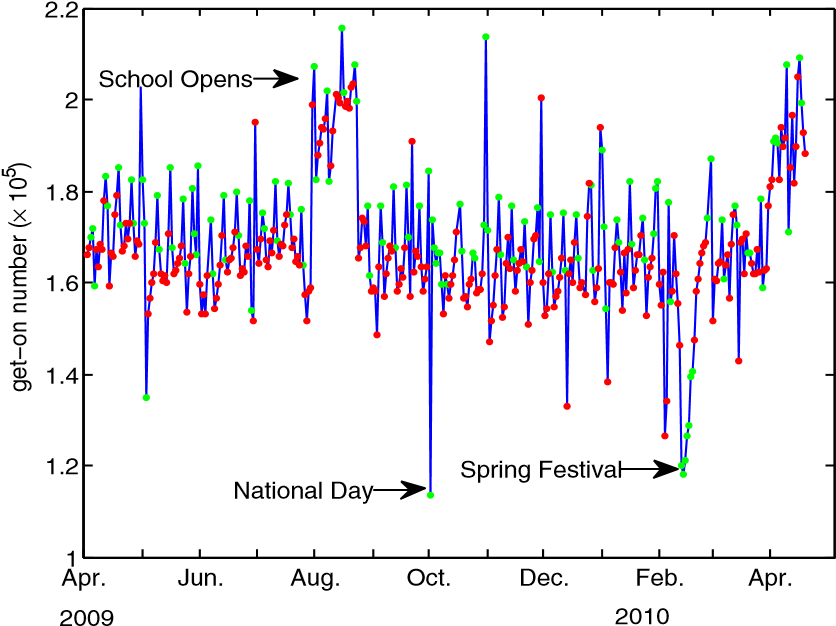
\includegraphics{fig/f1.png}
    \caption{Illustration of city-wide dynamics: total get-on/off amount variation over different days.}
    \label{fig:my_label_1}
\end{figure}

\subsection{Regional Social Functions Analysis}Besides the city-wide analysis, statistics of region-wide in a city may also exhibit patterns of human activity in the area. By qualitatively analyzing get-on/off amount in several time periods in a day, we observe that regions with different social function have their distinctive temporal variation patterns.
This paper preliminary considers three typical categories of regions: (1) coach/train stations; (2) entertainment districts; (3) scenic spots. Fig. 2 illustrates: • Train stations: Train stations are very hot in almost all the time over the whole day.


\begin{itemize}

\item Scenic spots: Tourists often go to scenic spots only during the daytime.
\item Entertainment districts: People usually go for entertainment mainly at night; few people will go there at dawn and seldom any passengers travel there in the morning.

\end{itemize}

The analysis above confirms relationship between regional taxi get-on/off amount and social activity in a region. The features of three types of regions we got by qualitative analysis conform to common sense. They show that taxi passengers are a kind of representative samples from citizens, and taxi get-on/off amount depicts human activity strength in a region. Besides, these examples show very different features of geton/off amount temporal variation for different types of regions, and hence the feasibility of recognizing social function of regions using temporal variation of get-on/off amount.
%%%%%%%%%%%%%%%%%%%%%%%%%%%%%%%%%%%%%
\section{SOCIAL FUNCTION RECOGNITION FOR REGIONS}%第五章
Section IV confirms qualitatively the relationship between regional get-on/off amount and human activity intensity. In this section, we analyze quantitatively the relationship between get-on/off amount and regions’ social function. With a simple classification method, we recognize precisely regions’ social function and find corresponding get-on/off amount time domain patterns.
\begin{figure}[htpb]
    \centering
    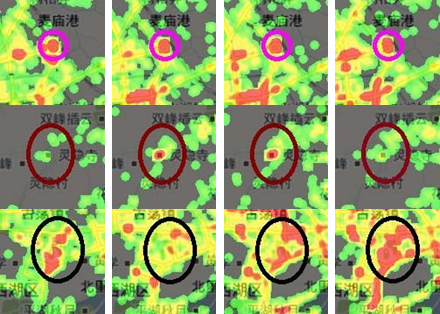
\includegraphics{fig/f2.png}
    \caption{Illustration of variation of passengers get-off number over time for three region categories. The grayscale of color represents density of get-on/off number. Each row is for one region category: train station, scenic spot and entertainment districts (from top to bottom).}
    \label{fig:my_label_2}
\end{figure}
\subsection{Data Labeling} For data preparation, we find three taxi drivers to label typical regions of each category with pure social function. We finally get 76 regions with pure social function in total and use them for further analysis. The labeled regions include 37 regions near train/coach station, 27 entertainment districts, and 12 scenic spots.
\subsection{Recognition of Social Function}Two types of features are considered: coarse-grained feature and fine-grained feature. Given n days data, the coarse-grained feature is a n-dimension vector with daily total amount of geton/off as element. The fine-grained feature is a 4n-dimension vector with four get-on/off numbers for four time periods in each day: (a) 6:30 a.m. to 8:30 a.m.; (b) 9:00 a.m. to 3:00 p.m.; (c) 7:00 p.m. to 9:00 p.m.; (d) 11:00 p.m. to 1:00 a.m. These four time periods are extracted according to the largest variance of amount. The recognition process is as follows:

\begin{itemize}

\item Feature Vector: The feature vectors are defined as $ x^{i}_{d} $ and $ x^{i}_{u} $ which represent the amount of get-on or get-off in the $i$th region $D_i$ with elements $ x^{i}_{u}(j) $ and $ x^{i}_{d}(j) (j=1,2,...) $.
\item Normalization: Normalization is to centralize the feature vector $ x^{i}_{u}(j)=x^{i}_{u}(j)-\Sigma_{j}x^{i}_{u}(j)/n $, and $ x^{i}_{d}(j)=x^{i}_{d}(j)-\Sigma_{j}x^{i}_{d}(j)/n $.
\item Similarity definition: We define similarity $ s_{i,j} $ between each two regions $ D_i $ and $ D_j $: $ s_{i,j}=max(cos(x^{i}_{u},x^{j}_{u}),cos(x^{i}_{d},x^{j}_{d})) $, where $ cos(x^i,x^j) $ is the cosine similarity of the two normalized vectors: $ x^i $ and $ x^j $.
\item Agglomerative clustering[10]: Agglomerate samples with enough large similarity (similarity threshold) into the same cluster. Some samples may be not much similar (similarity below the threshold) to the clusters and thus belong to none of the clusters. These samples are classified according to the most similar sample in clusters.
\item Recognition: Test samples are clustered together with training samples as above. Label the test sample according to voting by the number of training sample in the same cluster.

\end{itemize}

\subsection{Experimental Result and Analysis}

\subsubsection{Feature vector visualization}The coarse-grained feature vector extracted from one year data is visualized in Fig. 3
\begin{figure}[htbp]
    \centering
    \subfigure[]{
        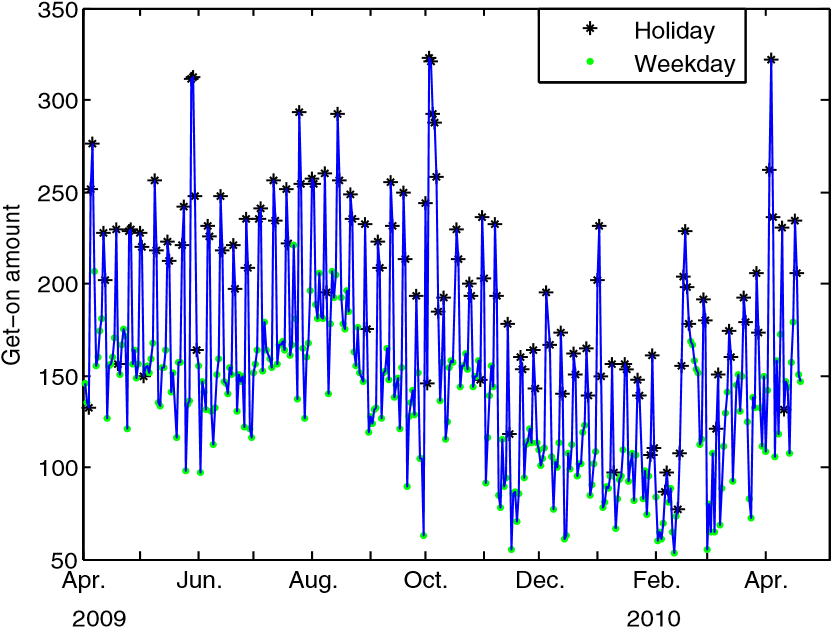
\includegraphics{fig/f3.png}
    }
    \subfigure[]{
        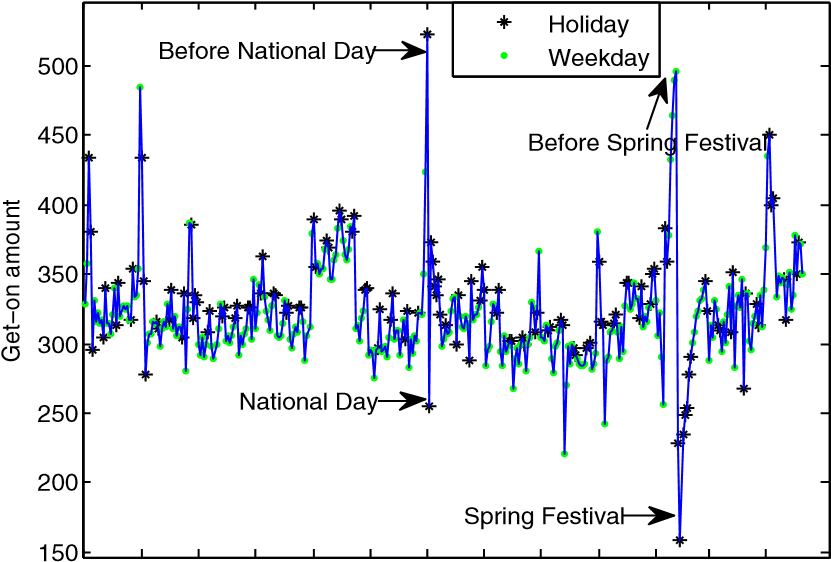
\includegraphics{fig/f4.png}
    }
    \subfigure[]{
        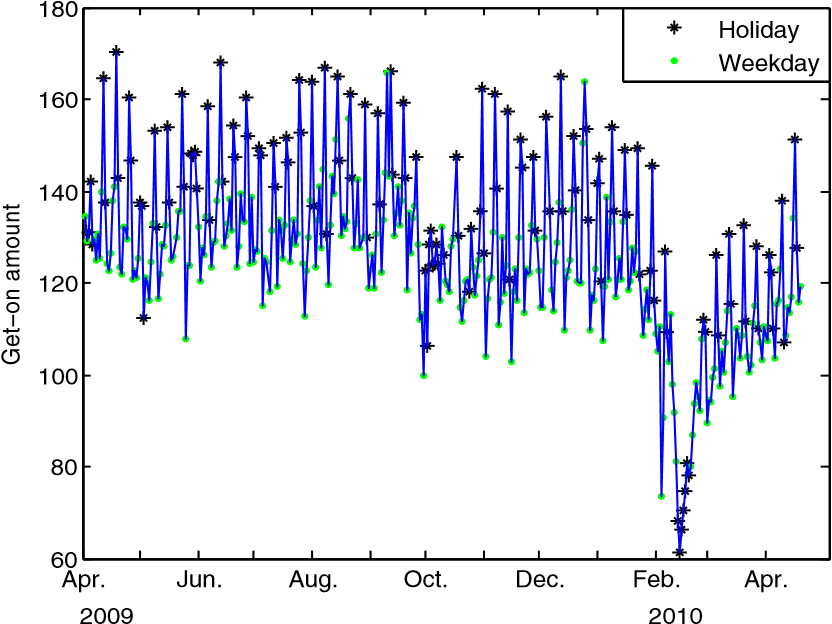
\includegraphics{fig/f5.png}
    }
    \caption{Visualization of feature vectors for the three region categories (a) scenic spots, (b) stations and (c) entertainment districts. All the get-on number is averaged over the regions of the same category.}
    \label{fig:my_label_3}
\end{figure}

\begin{itemize}

\item Train/coach station. Get-on/off amount of stations highlights some uncommon time points instead of difference between workdays and weekdays (Fig. 3b).
\item Entertainment districts. They are similar to scenic spots but the variance between the peaks and the troughs is small (Fig. 3c).

\end{itemize}

We also reduce the dimension of feature vectors by the principal component analysis and visualize the regions in the 3D-Eigenspace. In Fig. 4, samples with different region categories scatter apart from each other.

\begin{figure}[thbp]
    \centering
    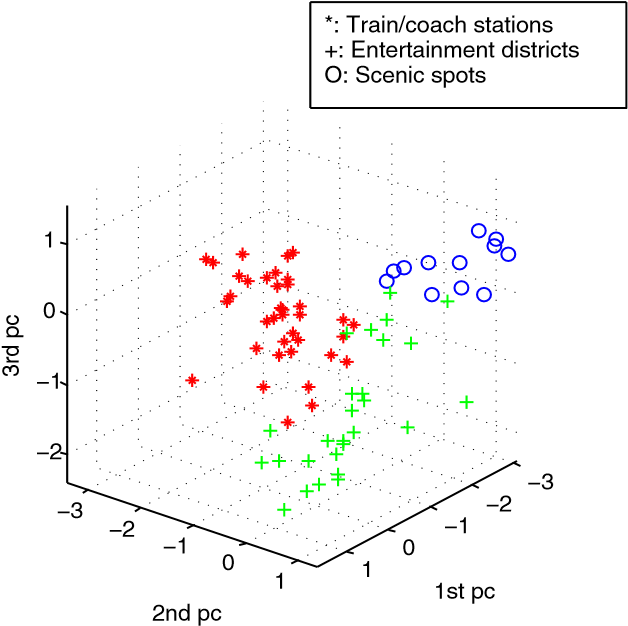
\includegraphics{fig/f6.png}
    \caption{Illustration of the labeled samples of three typical region categories in the 3D Eigenspace.}
    \label{fig:my_label_4}
\end{figure}


\subsubsection{ Recognition result and analysis}The recognition result is listed in Table I. Our method can recognize social function of the regions precisely. Moreover, there are some interesting conclusions we can get from this result: The tow types of features can be recognized more precisely with more data added. The recognition accuracy using coarse-grained feature grows quickly 5, while the accuracy using fine-grained feature changes slowly.

\begin{figure}[htbp]
    \centering
    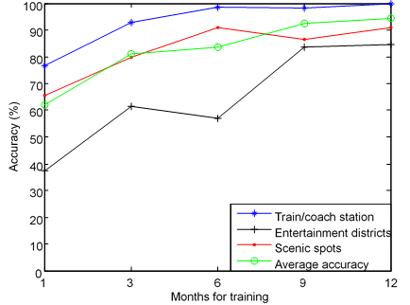
\includegraphics{fig/f7.png}
    \caption{Recognition performance of coarse-grained feature with varying data amount for training.}
    \label{fig:my_label_5}
\end{figure}

\begin{itemize}
\item For short time-span data (one week and one month), fine grained feature vector can be recognized more precisely since it considers different time periods during a day. For long time-span data (one year), coarse-grained feature vector has higher recognition accuracy.
\item The coarse-grained feature vector extracted from one year data can be best recognized. The average recognition accuracy using this feature is 94.44\%.

\end{itemize}

The results show that regions’ social function can be recognized correctly and these regions have clear temporal patterns. To sum up, by recognition, we reveal that, from a quantitative view, social function and regional get-on/off amount are indeed tightly related.

\section{CONCLUSION AND FUTURE WORK}%第六章
This paper investigates the relationship between regional get-on/off amount and regions’ social function. Firstly, from a city scale, the get-on/off amount variation in a day or among different days conforms to social activity intensity of citizens. Secondly, from a qualitative view, regional get-on/off amount daily variations are very different in regions with different social functions.
Based on the investigation, we develop a simple method to recognize regions’ social function. The preliminary results on a large-scale real-world taxi GPS data set show that our approach achieves recognition accuracy of 94.44%.
There is still much further work to do in the work-inprogress. Firstly, our regions are rigid squares which may not represent a intact region in the city. Thus, we are going to develop new methods to get more natural regions. Secondly, we consider only three types of regions. More social function classes should be added and more regions should also be considered. Finally, we consider regions with pure social function in this paper while regions are more complicate in reality.

\addtolength{\textheight}{-12cm}   % This command serves to balance the column lengths
                                  % on the last page of the document manually. It shortens
                                  % the textheight of the last page by a suitable amount.
                                  % This command does not take effect until the next page
                                  % so it should come on the page before the last. Make
                                  % sure that you do not shorten the textheight too much.

%%%%%%%%%%%%%%%%%%%%%%%%%%%%%%%%%%%%%%%%%%%%%%%%%%%%%%%%%%%%%%%%%%%%%%%%%%%%%%%%
\section*{ACKNOWLEDGEMENT}

This work is supported by the National High-Tech Research and Development (863) Program of China (No. 2009AA01190), the HGJ Program (2009ZX01039-001-002004, 2009ZX01038-002), the NSF of China (60803109), the Fundamental Research Funds for the Central Universities.

\begin{thebibliography}{99}

\bibitem{c1} G. O. Young, ÒSynthetic structure of industrial plastics (Book style with paper title and editor),Ó 	in Plastics, 2nd ed. vol. 3, J. Peters, Ed.  New York: McGraw-Hill, 1964, pp. 15Ð64.
\bibitem{c2} W.-K. Chen, Linear Networks and Systems (Book style).	Belmont, CA: Wadsworth, 1993, pp. 123Ð135.
\bibitem{c3} H. Poor, An Introduction to Signal Detection and Estimation.   New York: Springer-Verlag, 1985, ch. 4.
\bibitem{c4} B. Smith, ÒAn approach to graphs of linear forms (Unpublished work style),Ó unpublished.
\bibitem{c5} E. H. Miller, ÒA note on reflector arrays (Periodical styleÑAccepted for publication),Ó IEEE Trans. Antennas Propagat., to be publised.

\end{thebibliography}

\end{document}